\subsection{{\vfreename} Design}
\label{vfree:sec:design}
{\vfreename} is a modification to existing IO memory protection mechanisms
    for {\it strict} intra-VM protection in virtualized environments. {\vfreename} targets the same threat model as Linux strict mode (Appendix~\ref{vfree:sec:threat_model}).
%    that makes strict IO memory protection feasible in virtualized environments.
{\vfreename} achieves this goal using {\em One-for-Many Invalidations} (\S\ref{vfree:ssec:one-to-many}) 
    and {\em Deferred Free Page} (\S\ref{vfree:ssec:dfp}). % This section presents these two ideas.
% the two core design ideas in {\vfreename}: one-for-many invalidations and deferred free page.



% \subsubsection{{\vfreename} Overview}

% % As illustrated in Figure~\ref{vfree:fig:current-design}, the root cause of the performance inefficiencies in existing stacks is serialization of IRs across all threads in the VM. Keeping just one IR in-flight to the IOMMU HW for processing significantly reduces the achievable IO throughput, due to large IR processing latencies (owing to unavoidable VM exits in the datapath; \S\ref{vfree:sec:background-datapath}). In this section, we argue that such a serialized processing of IRs is in fact, completely unnecessary. And building on this insight, we propose {\vfreebrand}---a rearchitecture of memory protection mechanism for virtualized Linux network stacks---that enables concurrent IR processing, while providing strict memory protection. {\vfreebrand} thus helps achieving close-to-no-protection performance (\S\ref{vfree:sec:eval}), while still maintaining the strongest safety guarantees providing by existing stacks (\S\ref{vfree:sec:security}). 


% % {\vfreebrand} achieves its benefits by using two key design ideas, that are complementary to each other. The first idea---Safely Batched Invalidations (SBI)---enables concurrent IR processing by multiple vCPUs in the VM; and the second---Deferred Free Pages (DFP)---enables each vCPU to also concurrently submit multiple IRs for processing. \S\ref{vfree:sec:eval} evaluates the benefits enabled by each idea, and demonstrates that both are necessary to provide near-optimal performance. 

% % SBI is enabled by 



% % % enables concurrent IR processing by enabling each vCPU across the guest to concurrently submit an IR to the IOMMU. 
% % This is enabled by two key ideas: (i) using per-vCPU virtual queues for SW submission queue for safely performing concurrent IR-PREP (ii) decoupling IR-PREP and IR-SUB, to enable batching of multiple concurrent IRs to be submitted via IR-SUB which still needs to be serialized across cores. 

% % % While the first design alleviates the gap between no vIOMMU and strict protection performance, by improving concurrent IRs, specifically 1 by each vCPU, but that's not enough, given the high IR processing latency due to involved VM exits. 


% % The key challenge lies in maintaining strict memory protection under concurrent IR processing. 

% % The second design idea---deferred page frees---enables each vCPU to keep multiple concurrent IRs to the IOMMU HW, enabling to offset the high IR processing latency. This is enabled by performing invalidations asynchronously with unmaps. Performing this without impacting safety is based on the following insight: as long as the following ordering
% % of operations->unmap->invalidate→free page is followed, we
% % maintain the default strict protection guarantees, irrespective
% % (8) We argue this problem is not fundamental: \textit{contrary to conventional wisdom, executing both IR-PREP and IR-SUB synchronously with unmap calls are in fact NOT fundamentally necessary to achieve the strict memory protection.} This tradition fallacy arises due to the way existing network drivers recycle physical physical pages after unmap operations, to be mapped to other IO virtual addresses. The drivers today free a physical page after every unmap call. To ensure strict protection, we need to invalidate the IOTLB before the physical page is freed and recycled (or else it could result in known confidentiality attacks~\cite{}). Therefore, today invalidations are performed synchronously with unmaps to ensure they are always executed before the corresponding page free operations. Our key insight is that \textit{as long as the following ordering of operations---unmap$\rightarrow$invalidate$\rightarrow$free page is followed, we maintain the default strict protection guarantees}, irrespective of the fact whether invalidations are synchronous with the unmaps. \saksham{probably need to mention somewhere that recent linux kernel designs also ensure that there is no possibility of TOCTOU attacks even with asynchronous unmaps and invalidations.}
% % of the fact whether invalidations are synchronous with the unmaps. 

% % /** Current System */

% % lock (cache\_lock) // per domain

% % SUBMIT INV req to SW queue

% % lock (q\_lock) // per device

% % pick the request from the SW q and send to the HW q

% % PROCESS INV req

% % unlock(q\_lock)

% % unlock(cache\_lock)


% % /** Our Work */
% % // change per-domain cache\_lock to per-CPU cache\_lock

% % // change per-domain SW queue to per-CPU SW queue

% % // remove nested locking

% % lock(cache\_lock) // per CPU

% % SUBMIT INV req to SW queue

% % unlock(cache\_lock)

% % lock(q\_lock)

% % pick the request from the SW q and send to the HW q

% % PROCESS INV req

% % unlock(q\_lock)

% % \rachit{are we sure the above is correct?}
% % \subsubsection{Thoughts/Flow}

% % we decouple IR-PREP and IR-SUB; 

% % if we don't decouple, nothing fundamentally changes---we don't reduce the number of VM exits; 

% % \subsubsection{Preparing Invalidation Requests {\em Before} Cross-Core Serialization [\saksham{Will get rid of this subsection}]}

% % \begin{itemize}
% %     \item We want to reduce number of VM exits per unmap; today it is strictly more than 1, due to cross-core serialization before IR-PREP---prohibiting any opportunity to ``batch'' IRs to be submitted to the hardware via a single write to the invalidation queue, i.e. a single VM exit \rachit{for each point being made here, there should be a direct subsection/paragraph in S3 that we should be able to point to;} \rachit{we are mixing the goal with the solution: do not bring up batching; that is part of the solution}

% %     \item Such cross-core serialization today is performed to prevent concurrent reads and writes to per-IO-domain data structures; reads are performed during IR-PREP operation, writes are performed to allocate/deallocate the data structures during IO device attach/detach events. \rachit{could we point back to S2 where we discuss these?}

% %     \item We argue that performing cross-core serialization {\em before every} IR-PREP operation is unnecesarily aggressive, due to two reasons: (i) while concurrent reads and writes need to be serialized, there is no need to serialize concurrent reads; and (ii) attach/detach are rare events 

% %     \item We propose eliminating the cross-core serialization before IR-PREP, and only serialize reads and writes: {\em only when} attch/detach is happening, no thread can perform IR-PREP; otherwise concurrent threads can perform IR-PREP; since writes are rare events in practice, we most often see no serialization/blocking across cores to perform concurrent IR-PREP. \rachit{this is a bit confusing and if written this way will introduce questions related to safety guarantees: I suggest to describe it as {\vfreebrand} introducing a slow path and a fast path for IR-PREP: the former is triggered when attach/detatch happen and require cross-core serialization; the latter requires no cross-core seralization (common case)}  

% %     \item However, cross-core serialization is still required after IR-PREP: IR-SUB operation needs to be serialized---since it perfoms write to single emulated HW q (can't have multple emulated qs without modifyind the hypervisor); so serialization is necessary before IR-SUB; 

% %     \item Hence, our key design idea is to move cross-core serialization to after IR-PREP and before IR-SUB. Essentially, this design decouples IR-PREP and IR-SUB operations---i.e., they are no longer performed within the critical section of a same lock. Cross-core lock is only acquired before IR-SUB operation. 

% %     % \item If we need to reduce the number of VM exits per unmap, we need to perform a single VM exit for multiple IRs; that necessitates decoupling IR-PREP and IR-SUB; 

% %     % \item After concurrently preparing IRs, cross-core serialization is done to enqueue the requests to a single logical SW Q---enabling "batching" (need to be careful with the term); 
% % \end{itemize}
% % \rachit{high-level feedback: IR-PREP overheads do not even show up in Figure 6 and 7: why are we spending so much time and real estate discussing IR-prep?}

% {\vfreename} enables multiple vCPUs to concurrently prepare IRs for submission to the IOMMU; the vCPUs then remain blocked until invalidation is completed. For all invalidations requests concurrently prepared across different vCPUs, {\vfreename} enables actually submitting only a single IR descriptor to the IOMMU hardware in a manner that executing the single submitted invalidation request results in invalidating the IOMMU cache entries for all invalidation requests. Recall that submitting an IR descriptor to the emulated invalidation queue results in an unavoidable VM exit. Hence, using a single submission for multiple IRs reduces the number of VM exits to only one for entire set of concurrent requests (instead of one VM exit for each individual request as today). 

% We use two key insights to realize one-for-many invalidations. The first insight is to decouple the IR processing pipeline (IR-PREP and IR-SUB operations discussed in \S\ref{vfree:sec:background-datapath}) across multiple threads, each using separate independent locks. This allows multiple vCPUs to concurrently perform IR-PREP operations to prepare requests while IR-SUB is concurrently executing on another thread. The second insight enables performing invalidation for the multiple prepared IRs using only a single submission to hardware. We achieve this by sending an IR with a special flag that {\em flushes all IOMMU caches} for the VM. While flushing the IOMMU caches can increase address translation overheads (due to larger IOPT lookup overheads owing to IOMMU cache misses~\cite{Rubin2024FastSafe}; \S\ref{vfree:sec:background-datapath}), increasing address translation overheads to reduce the number of VM exits turns out to be a good tradeoff. 

% While one-to-many invalidations enable multiple vCPUs to concurrently prepare IRs, each vCPU still remains blocked upon preparing a single IR until invalidation limiting the performance benefits. This is done to guarantee strict safety since the IOVA and the corresponding physical page must be released for future reuse only after completing invalidation. {\vfreename}'s second design idea of deferred free page addresses this challenge: {\vfreename} ensures that each page is freed only after the corresponding invalidation has been completed. Using this idea, vCPUs are not blocked and can continue preparing more IRs even while the previous IRs have not been invalidated. The key insight here is as that long as physical pages are freed only after their corresponding IOVAs are invalidated, strict safety is guaranteed. 

% The next two subsections describe the two ideas in detail; we then discuss how {\vfreename} maintains strict safety guarantees (\S\ref{vfree:sec:security}).

% \begin{itemize}
    


%     his is because, to
% guarantee strict safety, the IOVA and the physical page must
% be released for future use only after the invalidation has
% completed [? ? ? ]. To that end, the deferred free page idea
% delegates free IOVA and free page operations to the dedi-
% cated vCPU, which performs these operations only and im-
% mediately upon receiving the completion signal.

    % \item The second idea is deferred free page
% \end{itemize}
\subsubsection{Enabling Concurrent Invalidation Requests}
\label{vfree:ssec:enabling}
As discussed in \S\ref{vfree:sec:background-datapath}, 
    existing IO memory protection mechanisms 
    enforce strictly one invalidation requests (IR) in flight: 
    vCPUs acquire the \CodeIn{cache\_lock} before executing IR-PREP, 
    synchronously execute IR-SUB, and release the lock only after the IR completion signal is received; 
    during this process, all other vCPUs remain blocked, waiting to prepare and submit their respective IRs. 
Since each IR requires a VM exit, existing IO memory protection mechanisms 
    enforce at least one VM exit per IR to enable strict IO memory protection.

\para{Fast path for concurrent IRs.}
{\vfreename} enables a fast path within IO memory protection mechanisms that 
    allows keeping multiple in-flight IRs. 
To achieve this, {\vfreename} decouples the two operations involved in IR processing---preparing 
    IR descriptors (IR-PREP) and submitting the descriptors to the hardware (IR-SUB)---across multiple threads. 
Specifically, {\vfreename} uses a producer-consumer model, as shown in Figure~\ref{vfree:fig:async-design}. 
IR-PREP is executed by producer threads---which are the same threads performing unmap operations. 
Furthermore, {\vfreename} replaces the single IO-domain queue and \CodeIn{cache\_lock} 
    with per-CPU virtual IO-domain queues, each protected with per-CPU \CodeIn{cache\_locks}. 
This allows multiple producer threads (running concurrently on multiple vCPUs) 
    to concurrently execute IR-PREP: 
    each producer acquires its per-CPU \CodeIn{cache\_lock}, 
    prepares an IR, enqueues it in per-CPU virtual IO-domain queue, releases the per-CPU \CodeIn{cache\_lock}, and then waits to receive a completion signal for its IR. 
With this design, multiple IRs can be kept in flight. %producer threads across vCPUs can now concurrently execute IR-PREP. %In fact, our measurement results in Figure~\ref{vfree:fig:lock-contention} establish that IR-PREP is a light-weight operation. To run IR-PREP, the thread first acquires the \CodeIn{cache\_lock}, enqueues the prepared IR descriptor in the {IO-domain queue}, and then immediately releases the \CodeIn{cache\_lock}.

The IR-SUB operation is executed by a consumer thread on a designated core. % (the highest-numbered online core).
% For design simplicity, the consumer thread runs on a dedicated vCPU by default (we discuss an optimization in \S\ref{vfree:sec:impl} 
%    that allows the consumer thread to run in a distributed manner without any dedicated vCPU). 
The consumer thread acquires each per-CPU \CodeIn{cache\_lock} one at a time, 
    copies pending IR descriptor(s) from the per-CPU IO-domain queue to a temporary buffer, 
    and immediately releases the per-CPU \CodeIn{cache\_lock}. 
%--- the IR-SUB operation always executes there.
% \review{
When a producer observes that its IR has not completed, 
    it attempts to activate the consumer by atomically test-and-setting a domain-wide BUSY bit.
If the test-and-set succeeds, the consumer is inactive; thus,
    the producer schedules the consumer on the designated core
    via a workqueue.
    % via a high-priority workqueue running in softirq context.%
% \footnote{We chose a workqueue over SMP function calls because the latter would execute in hard-interrupt context,
% which cannot invoke DFP callbacks with NAPI optimizations~\cite{linux_napi,mlx5_napi_poll} \rachit{we have not introduced DFP yet}}
If the test-and-set fails, the consumer is already running;
the producer spins on the completed counter until the consumer finishes.
If the producer is running on the designated core
(dispatching via the workqueue would deadlock), %since the target core is occupied by the producer itself.
    the producer executes the flush locally, bypassing the workqueue.


% \rachit{the rest of the paragraph should move to the next subsection}
% Only after processing all per-CPU virtual IO-domain queues, the consumer thread acquires the \CodeIn{q\_lock}, copies the descriptor from the buffer to the emulated HW queue. It then notifies hypervisor to perform invalidation by writing 
% to the MMIO invalidation queue tail register (incuring a VM exit); it releases the \CodeIn{q\_lock} only upon the invalidation completion. 

\begin{figure}[H]
	\centering
% 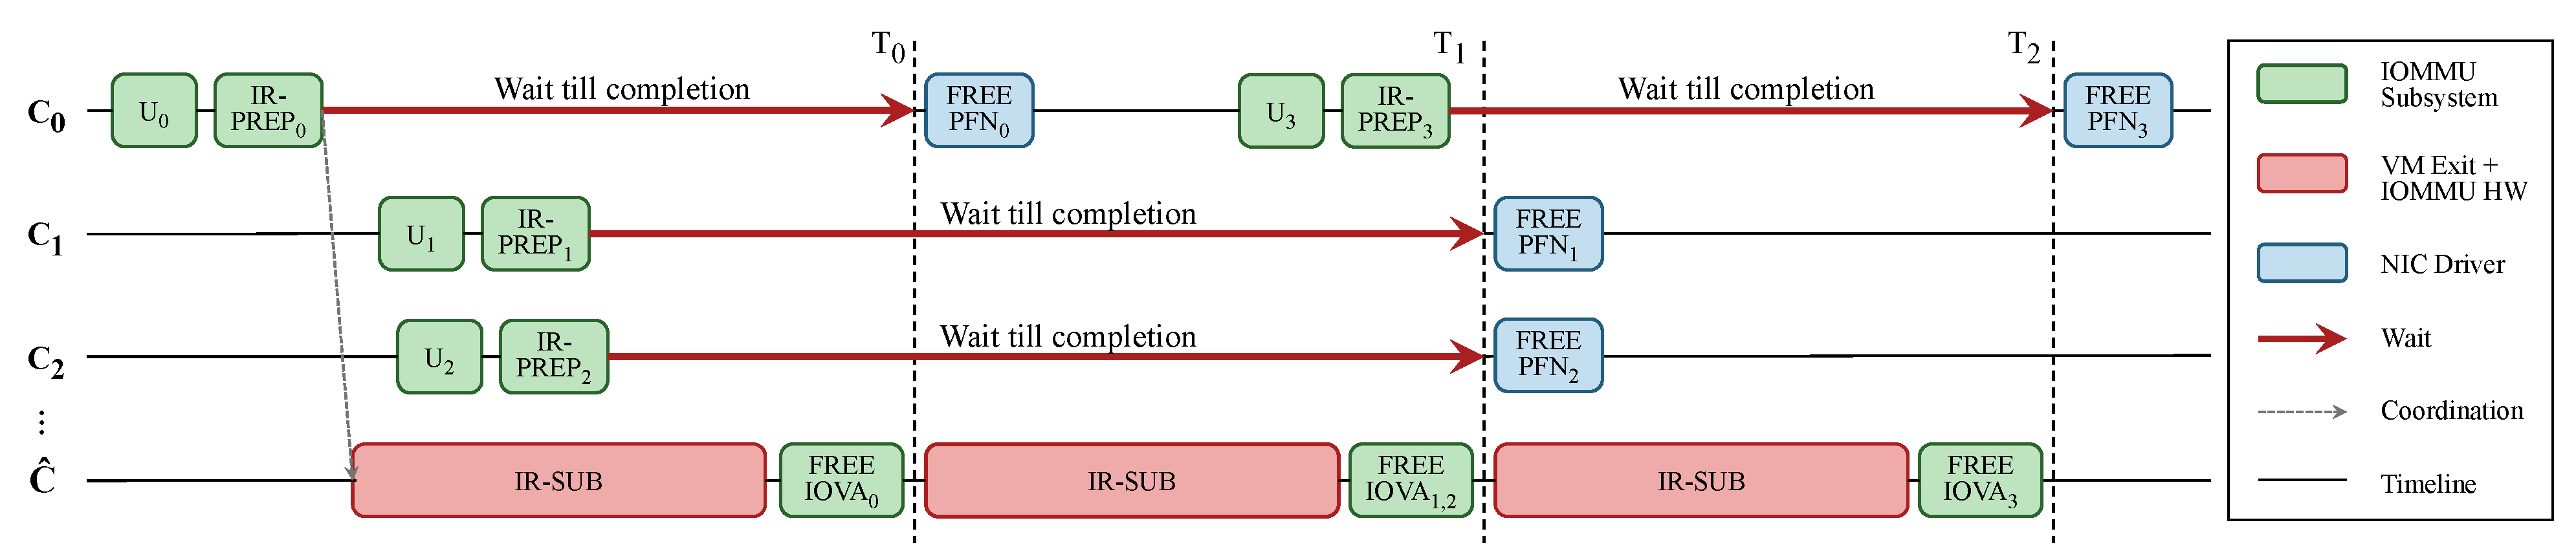
\includegraphics[width=\linewidth]{figures/omf_v4_cropped.pdf}
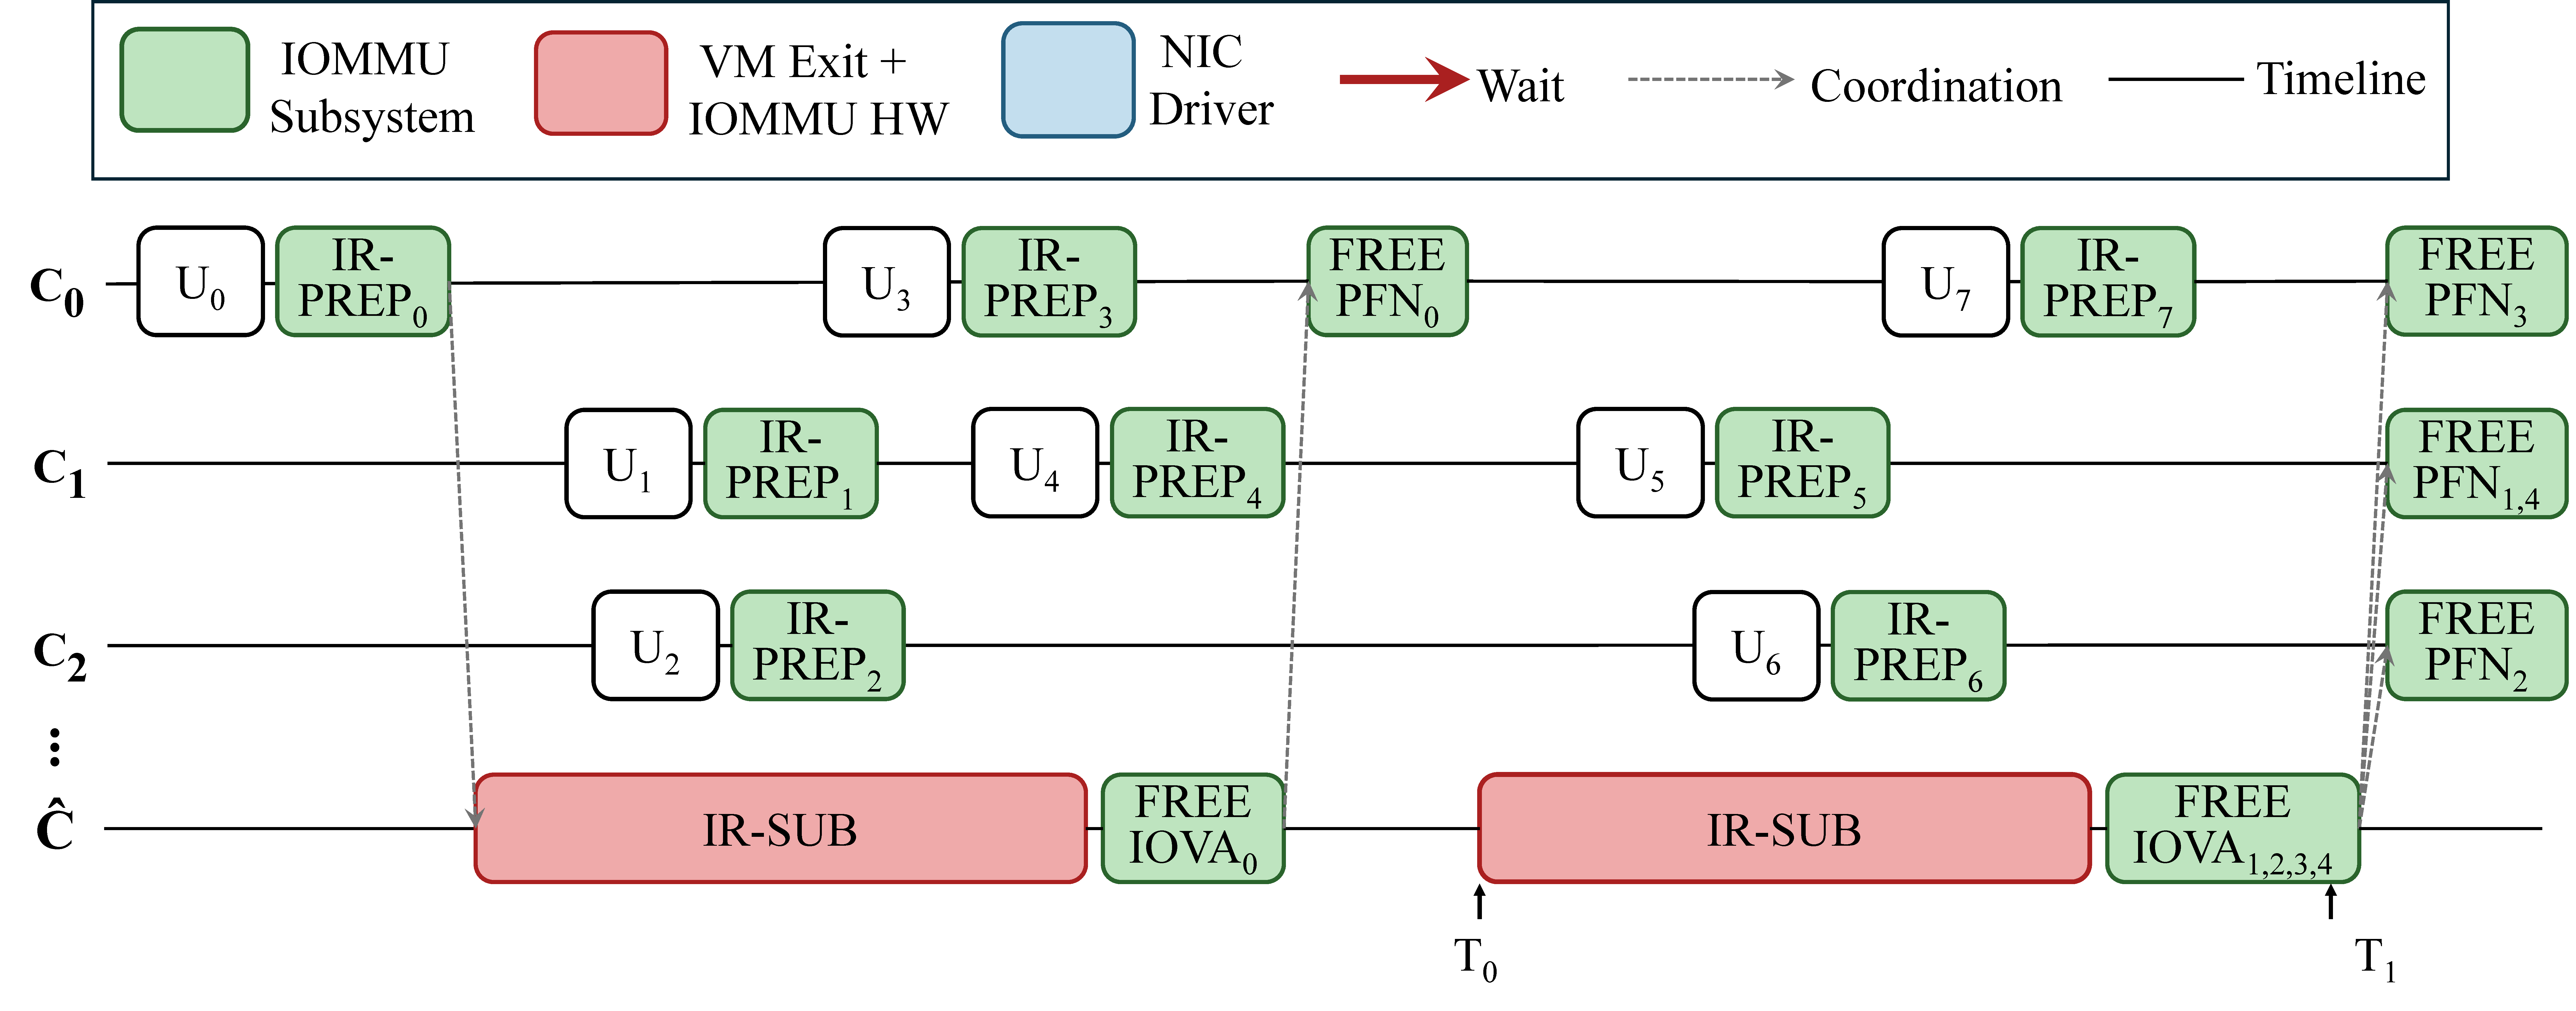
\includegraphics[width=\linewidth]{figures/One_for_many_timline.pdf}
\caption{\small
    \textbf{
One-for-many enables multiple IR-PREPs to run concurrently with an IR-SUB operation. 
It reduces the number of VM exits by using one IR-SUB operation
for all outstanding IRs to flush all IOMMU caches.}
In this figure, producers run on cores $C_1, C_2, C_3$, and a dedicated consumer thread runs on $\hat{C}$.
Each producer performs an unmap operation (U$_{1-3}$) and busy-waits until its IR is invalidated by the consumer thread.
}
% \saksham{We need to show the pinned version here instead; showing consumer thread running on 1 core, and producers on others; }\saksham{we should club copy as part of IR-SUB}}
\label{vfree:fig:async-design}
\end{figure}

% \para{Per-CPU queue for IR-PREP.}
% We improve the scalability of \vfreebrand
% by replacing the single IO-domain queue and \CodeIn{cache\_lock}
%     with per-CPU queues protected by per-CPU locks.
% % The per-CPU SW queue is protected by a per-CPU lock.
% The optimization enables multiple producers to execute IR-PREP in parallel.
% With the per-CPU queue,
% each producer acquires its per-CPU lock,
% prepares an IR and enqueues it.
% After the short IR-PREP (As shown in Figure~\ref{vfree:fig:lock-contention}), the producer releases the lock.
% This optimization avoids multiple producers contending for the per-IO-domain \CodeIn{cache\_lock} 
%     at IR-PREP time,
%     which could lead to long lock contention especially when DFP is enabled. \leshna{quick explaination as of why}

% The consumer copies all IRs from all per-CPU queues to a temporary buffer.
% It grabs the per-CPU lock one by one, and releases it after each copy.
% % The consumer never holds more than one per-CPU lock at a time.
% % it acquires the per-CPU lock,
% % rather than contending for the per-IO-domain \CodeIn{cache\_lock} a per-IO-domain SW queue.
% % The per-CPU SW 
% % % a per-CPU SW queue rather than a per-IO-domain SW queue.
% % After the producer core unmaps an IOVA, it acquires only its own per-CPU lock, prepares an the request based on given IOVA range, 
% % and appends the IR to its per-CPU SW queue.
% The per-CPU lock is released before IR-SUB,
%     enabling other producers to prepare more IRs while the consumer performs IR-SUB.

% \paragraphb{Slow path for maintaining strict IO memory protection}
\para{Slow path.}
As discussed in \S\ref{vfree:sec:inefficiencies}, IO memory protection mechanisms 
    use \CodeIn{cache\_lock} to protect cache tags for each IO-domain, as
    a domain can be attached/detached at any time, and the list of cache tags is recycled during invalidation.
% With our per-CPU design,
% This is a more expensive operation than acquiring a single per-IO-domain lock,
The domain attaching/detaching is a rare event, but must be accounted for to maintain strict IO memory protection. 
Thus, any domain attaching/detaching event triggers the slow path: \emph{all} per-CPU \CodeIn{cache\_locks} 
    have to be acquired at attaching/detaching time to ensure safety.

\subsubsection{One-for-Many Invalidations}
\label{vfree:ssec:one-to-many}
% \saksham{todo---we'll be mentioning one-for-many itself as the first key design idea; rethink how the two concepts below are introduced, not as two design ideas again}
% \saksham{Todo: avoid using the word "(a)synchronous"}
% \schaix{
% , and then releases the \CodeIn{q\_lock} upon receiving write completion.
% % }
% \schai{
% It then acquires the \CodeIn{q\_lock}, copies the descriptor from the buffer to the emulated HW queue, 

% The VM exit is triggered at MMIO write time.
% The MMIO write triggers a VM exit to doorbell the hypervisor 
% pass the invalidation request to host OS and utimately invalidating the physical IOTLB or IOPT caches.
% }
% followed by MMIO write to the invalidation queue tail register to 

% each preparing IR descriptors and enqueueing to a shared, per-IO-domain, \CodeIn{sw\_queue}. 

% Specifically, we propose performing IR-PREP and IR-SUB operations independently, in separately acquired locks 

% \saksham{todo: Some details on producer/consumer design here to enable decoupling; say IR-PREP is performed by the producer threads---same thread performing unmap, after IR-PREP; a dedicated consumer thread for IR-SUB, AND ALSO freeing the corresponding IOVAs}

% (shown in Figure~\ref{vfree:fig:decoupled-design}\saksham{Todo: add figure}).



% Such decoupled IR processing enables a useful design opportunity which can help reduce the number of VM exits per unmap. This is because the decoupled design allows concurrent 
Decoupling IR-PREP and IR-SUB processing across producer and consumer threads enables 
    {\vfreename} to execute them concurrently. 
Recall that the majority time of IR-SUB 
    is spent for the VM exit, 
    which is executed within the \CodeIn{q\_lock}; 
IR-PREP requires only acquiring the per-CPU \CodeIn{cache\_lock}, and can therefore be executed concurrently. 
Executing multiple IR-PREPs concurrently during an ongoing IR-SUB enables generating multiple IR descriptors 
    by the time this IR-SUB operation finishes. 
The one-for-many invalidations technique in {\vfreename} exploits this opportunity 
    to efficiently reduce the number of VM exits per unmap operation.

% This presents an opportunity to submit a single representative IR descriptor to the hardware that can collectively invalidate all IOVAs in the group of IRs.  %needed for invalidations from $N$ to 1. 
% \saksham{Do we need to discuss the tradeoff here, that we need to acquire the cache lock again to read the IR from SW Q to copy to HW Q, but its a good tradeoff to make due to reduced VM exits?}
    

\para{Flushing IOMMU caches to enable one-for-many invalidations.} 
The (emulated) IOMMU invalidation queue supports submitting 
    multiple IR descriptors---up to 256 entries in our setup---before updating the tail register. 
It is possible to use this interface to submit all outstanding IRs with a single tail register update (and hence a single VM exit); 
this will invalidate the IOMMU cache entries corresponding to the outstanding IRs. 
The invalidation queue in existing hardware only supports invalidating a contiguous IOVA range 
    for any enqueued IR descriptor~\cite{intel_scalable_iov_spec}. 
However, the group of IR descriptors to be invalidated can be arbitrarily discontiguous 
    collectively\footnote{Existing works~\cite{Rubin2024FastSafe} have studied reasons 
        for discontiguity in IOVAs allocated even for successive maps.}.
Thus, when submitting multiple descriptors together to the invalidation queue, 
    the total time to invalidate IOMMU caches will scale with the number of entries submitted. 
Specifically, IOTLB invalidation cost is known to be ${\sim}{600}$-${700}$ns~\cite{Malka2015rIOMMU}
% \saksham{Siyuan, might be nice if we can measure on our server}. 
Hence, the overhead of performing multiple invalidations, one for each outstanding IR, will at least be a few microseconds.

{\vfreename} executes only one IR for all outstanding IRs, 
    but invalidates the {\em entire} IOVA address space for each IR-SUB operation, 
    independent of the IR group size or IOVA ranges the IR group represents. 
This is feasible today via a special IR descriptor type that 
    {\em flushes} all IOMMU cache entries associated with the guest\footnote{IOMMUs today provide 
        per-guest isolation in caches by using separate PASIDs for each guest~\cite{Zhang2024HDIOV}}. 
% \saksham{Mention here we flush only the caches associated with the guest; there is per-guest isolation in terms of caches}
%
% submits a single representative IR descriptor to the IOMMU invalidation queue, along with a flag requesting the hypervisor to flush all IOMMU caches for the corresponding VM. we argue that flushing the IOMMU caches still provide a better trade-off. 
%
Flushing the IOMMU caches maintains correctness guarantees---\textit{i.e.}, the IOVAs represented by 
    the group of IRs will be invalidated. 
Thus, the submitted IR acts as a {\it one-for-many} invalidations: 
    the single submitted IR results in invalidating the IOMMU cache entries for all outstanding IRs. 
This reduces the number of VM exits by the same factor as the number of outstanding IRs. 
However, flushing the IOMMU caches also poses an inherent tradeoff: 
    while VM exits per unmap and invalidation decrease, the address translation cost may 
    increase (see phase 2 in \S\ref{vfree:sec:background-datapath}). 
This is because after flushing IOMMU caches, subsequent IOVA-to-HPA lookups may take as many as $4$ memory accesses, 
    instead of potentially $1$--$4$ depending on cache hit rates~\cite{Rubin2024FastSafe}. 
% \saksham{Revisit this given 2-level translation, and end-to-end translation, i.e., IOVA-to-HPA kept in IOTLB can also be lost; could be more than 3 extra accesses.}
This is a strictly good tradeoff to make: even in the extreme case 
    where we incur three extra memory accesses for address translation, 
    assuming a pessimistic memory access latency of $100$ns, 
    it will cost ${\sim}3\times100$ns extra overhead. 
This is much smaller than a VM exit overhead, which can be several $\mu$s (10--12$\mu$s in our measurements).  
Moreover, larger sized IR groups being invalidated using a single flush (which will be the case in the high network load case) result in larger gains. 
    % \vspace{0.1in}
    % \paragraphb{Using one-for-many invalidations in {\vfreename}}
    % We next describe how {\vfreename} builds upon the two key insights discussed above to minimize VM exits per unmap, while maintaining the same safety guarantees as strict memory protection in Linux. 

\begin{figure}[H]
	\centering
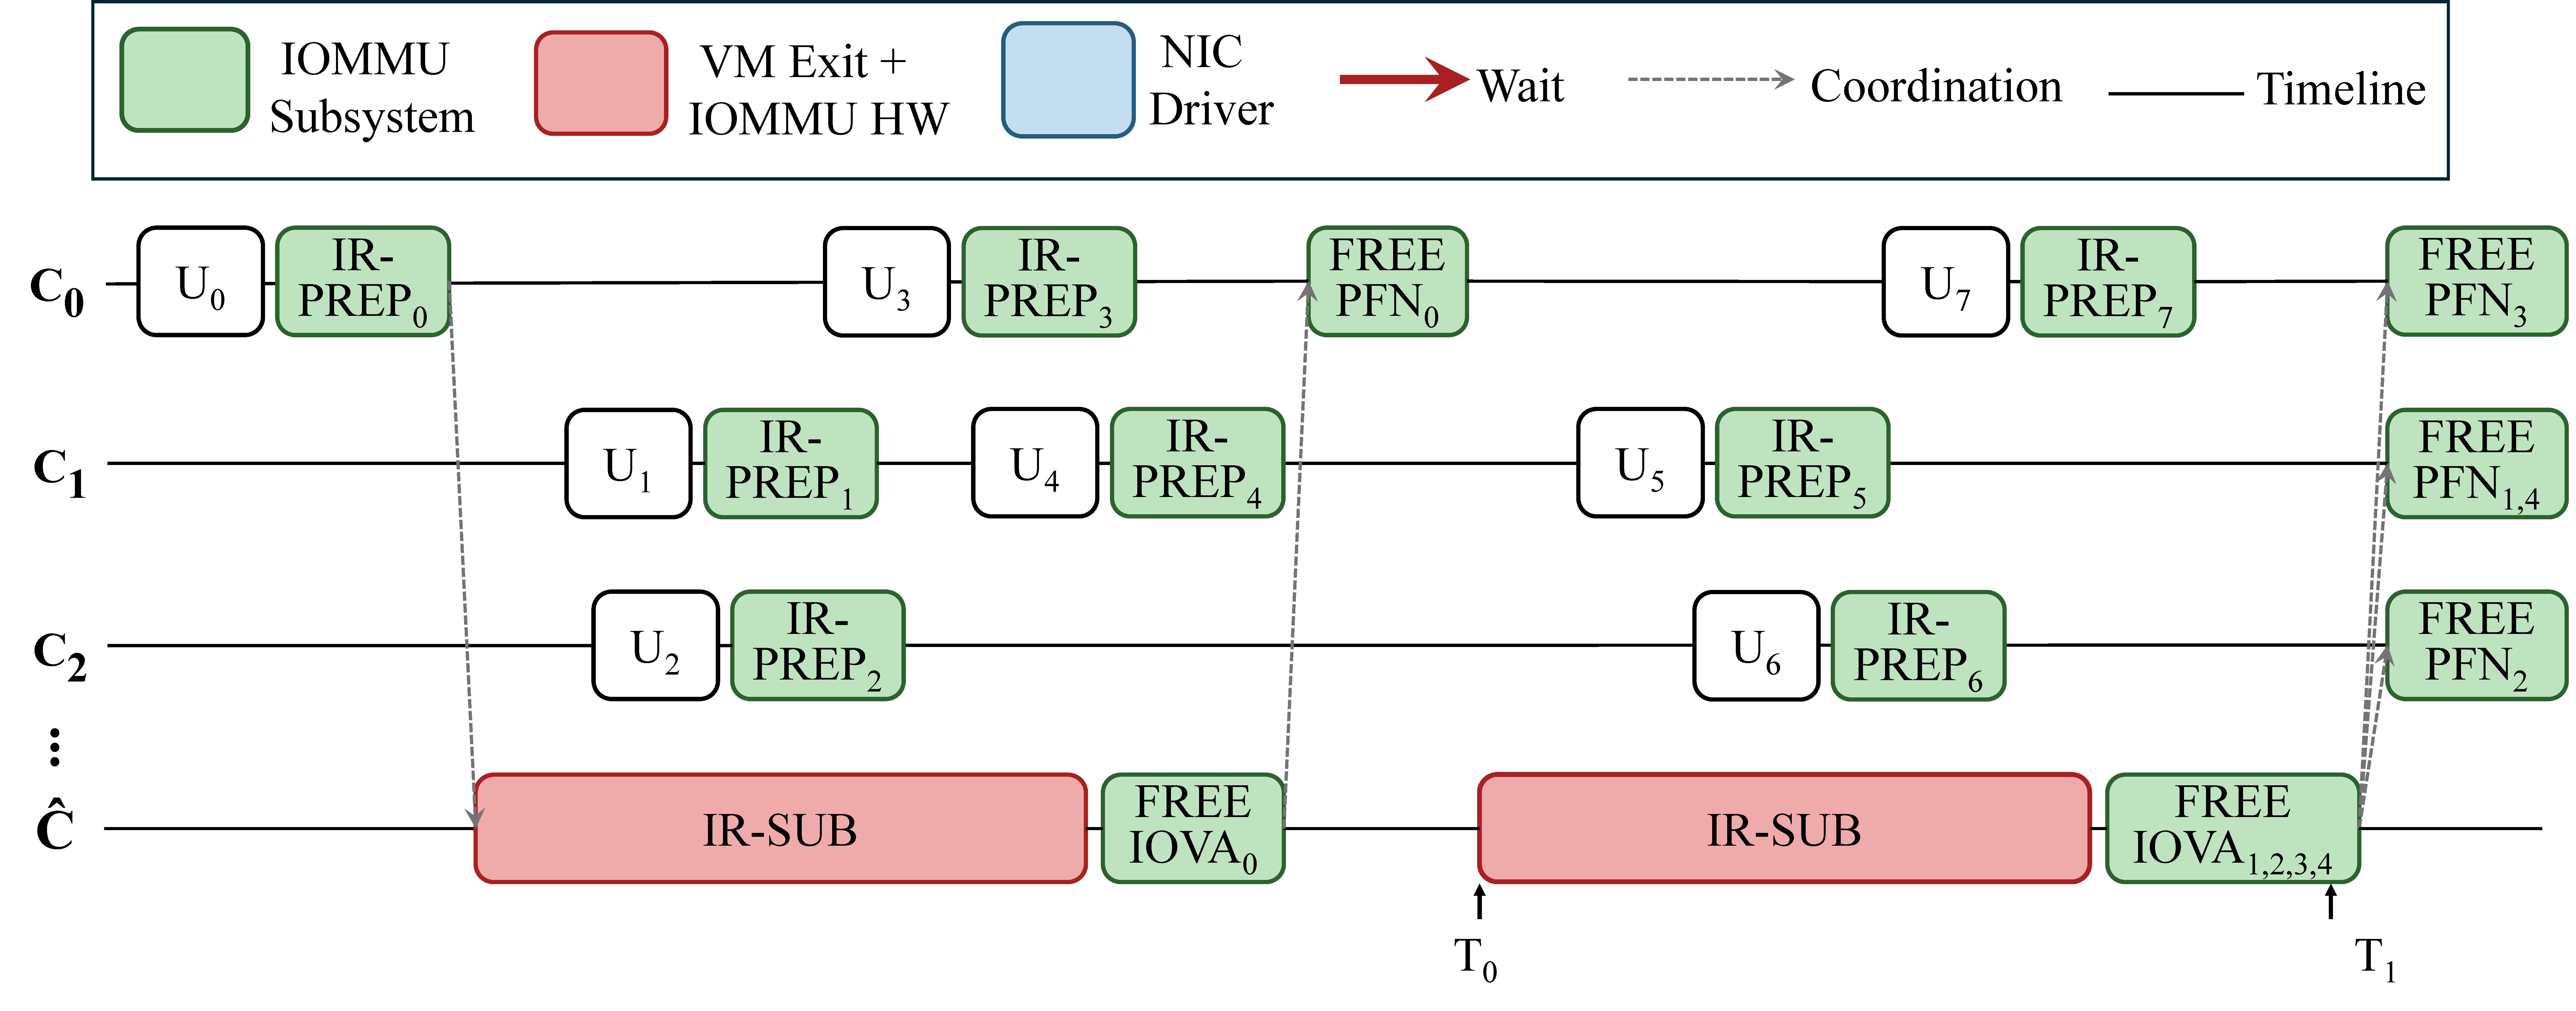
\includegraphics[width=\linewidth]{figures/dfp_timeline.pdf}
% 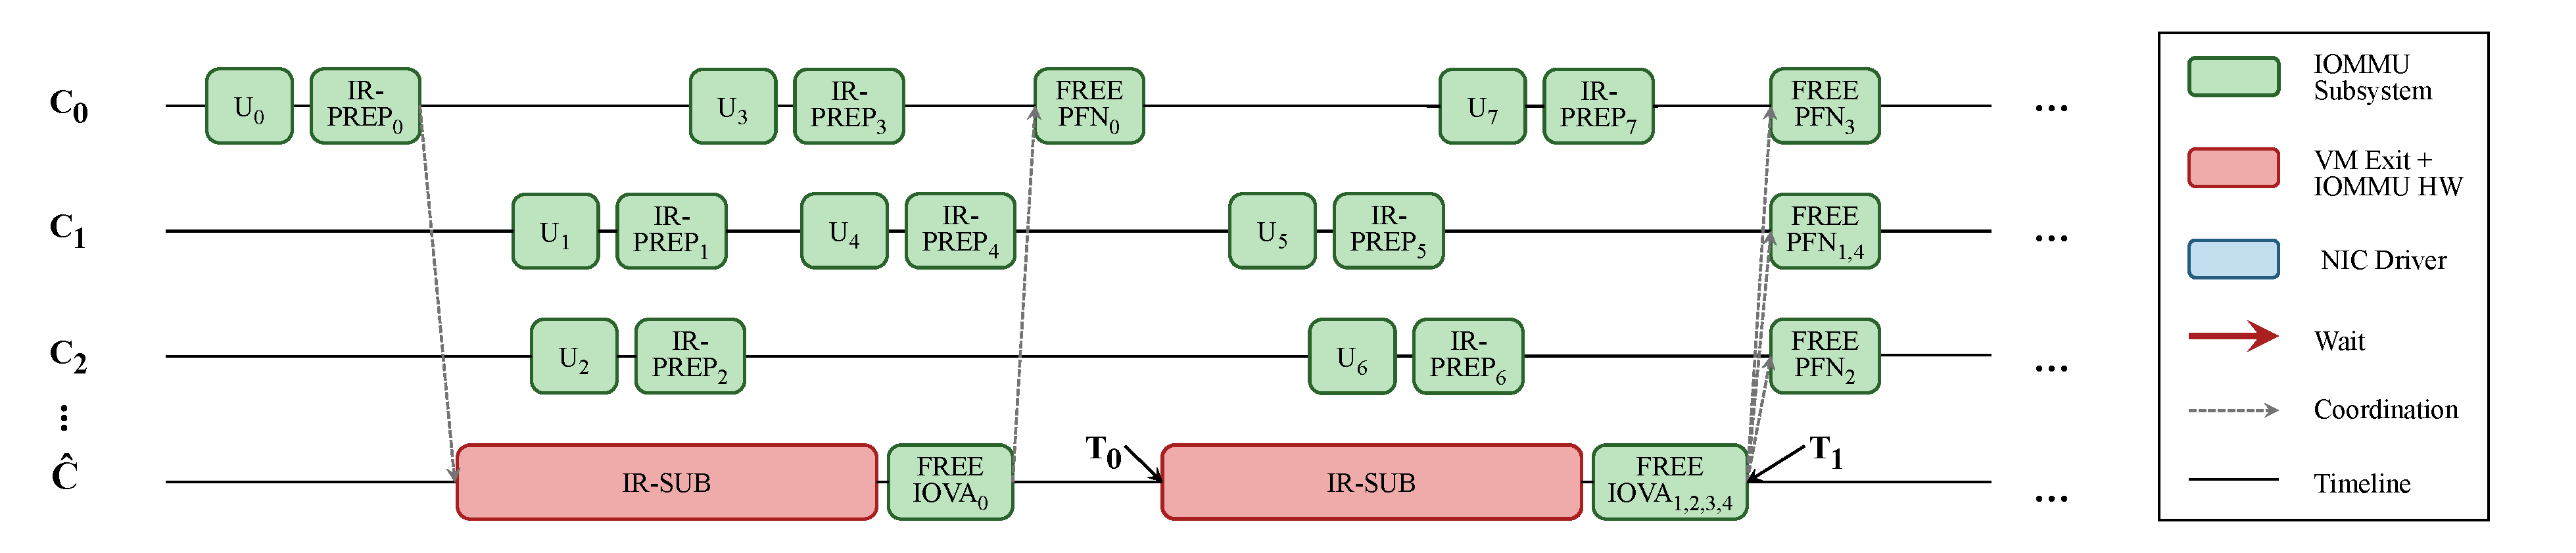
\includegraphics[width=\linewidth]{figures/dpf_side_cropped.pdf}
\caption{\small
    \textbf{
With deferred free page, vCPUs
can proceed immediately without waiting for the invalidation to complete.}
In this figure, producers run on cores $C_1, C_2, C_3$ and dedicated consumer runs on $\hat{C}$.
Each producer thread performs unmap (U$_{1-3}$) and IR-PREP operations and immediately proceed.
It enforces strict protection by deferring the free page operation to after the IR-SUB operation completes.
}
% \saksham{Copy is part of IR-SUB the way I've currently defined in text; one thing needs to update.}}
\label{vfree:fig:dfp}
\end{figure}

    % \paragraphb{An example}
Figure~\ref{vfree:fig:async-design} illustrates the one-for-many invalidation design: 
    each producer, upon any {unmap}, executes IR-PREP. Next, there are two cases. 
First, if the consumer thread is inactive (such as for {\tt IR\_PREP$_0$} in Figure~\ref{vfree:fig:async-design}), 
    % \schaix{the producer thread wakes up the consumer and asks it to perform IR-SUB.}
    {the producer thread schedules the consumer thread on a designated vCPU.} 
    % \schaix{Upon waking up,} 
    The consumer copies IR descriptors from each of the per-CPU virtual IO-domain queues, 
    acquires the \CodeIn{q\_lock}, copies one of the IR descriptors with the flush-all flag, 
    and then writes to the MMIO invalidation queues tail register (incurring a VM exit); 
    the consumer then busy waits until it receives the invalidation completion signal; 
    upon receiving the signal, it frees IOVAs contained in the IR descriptors copied from the per-CPU virtual IO-domain queues. 
Or,  
    % \noindent
    % (2) 
    if the consumer thread is active, running IR-SUB for previously prepared IRs (such as  {\tt IR\_PREP$_1$} in Figure~\ref{vfree:fig:async-design}), the IR will be submitted by consumer's next round of operations. When any round of consumer operations finishes, the consumer starts executing another round if there are any descriptors present in the per-CPU virtual IO-domain queues. 
    % \schaix{Otherwise, it goes to sleep.} 
    {Otherwise, it terminates.} 
    % \schaic{The change here doens't impact the design story, what I added is what we actually have.}

   
    % When the current IR-SUB operation finishes, 
    %     the consumer core collect all IRs from all producer cores' SW queues, perform a single IR-SUB (single VM exit) that flushes all IOPT caches for the domain,
    %     and free the IOVAs based on all IRs.
    % Otherwise, if an IR-SUB operation is ongoing concurrently, the thread remains blocked until the IR-PREP. 
    
    Importantly, each producer thread also {\em busy waits} until its IOVA has been successfully invalidated and freed by the consumer. For instance, producer thread $P0$ waits until time $T0$, and $P1,P2$ wait until time $T1$ in Figure~\ref{vfree:fig:async-design}. This is required to maintain strict IO memory protection with existing network drivers. The drivers today free a physical page after every unmap call (shown in blue color in Figure~\ref{vfree:fig:async-design}). To ensure strict protection, we need to invalidate the IOMMU caches before the physical page is freed and recycled; or else it could result in known integrity and confidentiality attacks~\cite{RajapakshaIOMMU}. 
    % \saksham{Come back here after reading safety subsection}
    % Therefore, today invalidations are performed synchronously with unmaps to ensure they are always executed before the corresponding page free operations---as is the case with this proposed design.
    
\para{Preserving strict IO memory protection.}
One-for-many invalidation preserves the invariant required for strict IO memory protection---each core still blocks until 
    its own invalidation request (IR) completes before freeing the page.
What changes is \emph{when} the invalidation descriptor is submitted to the IOMMU hardware, 
    {\it not} the order between IR completion and page free.
% Under vanilla strict mode, each core acquires the global lock, submits one invalidation descriptor, busy-waits for hardware acknowledgment, and only then proceeds to page free.
% Under \optOne, the core still submits its invalidation descriptor and still waits for hardware acknowledgment before proceeding---the difference is that the lock is released after enqueue rather than after completion, allowing multiple cores to have invalidations in flight concurrently.
The only relaxation is \emph{between} cores: one core's IR need not complete before another core enqueues its own.
This cross-core concurrency does not violate the invariant, 
    which holds per-page: a page is freed only after the invalidation that covers it has completed. 

% \schaic{is the cross-core concurrency a relaxation? How can previous IR's completion affect another core?}   
% no; see the invariant    

    
  

    

    % Try to perform as many IR-PREP as possible before the IR-SUB operation, to minimize the number of VM exits per unmap; but also not unnecesary delay the IR processing. 
    % waiting for longer to further aggregate IRs would result in inefficiency---unnecesarily delay the processing of an IR, degrading the throughput. 
    % why not wait for very large group size---try to submit IR as soon as possible, to minimize the average IR processing. 
    
    % \item Specifically, we propose the following design (as shown in Figure)---referred to as {\em Safely Batched Invalidations}: IR-SUB operations are serialized; IR-PREP operations from multiple cores execute concurrently, perform cross-core serialization after preparing the IRs to enqueue them to a single Q to form a group to be invalidated; whenever IR-SUB operation (invalidating previous group of IRs, by flush operation) gets free, it invalidates the next group of IRs. the IR-PREP threads busy wait until the current group of IRs is invalidated successfully by IR-SUB---i.e., within each thread, IR-PREP and IR-SUB operations are decoupled, but still synchronous. 
    % \schaic{I prefer the name "coalesced invalidation"}.

% \begin{itemize}
%     \item
%     % \schaic{I think we go way to high level here. Readers won't know what exactly happening if we just have previous paragraph.}
%     \schai{
        % Our design decouples IR-PREP and IR-SUB into different cores, a significant difference from vanilla implementation of strict protection.
        % We reshape the invalidation path with a producer-consumer model.
        % We have multiple producer cores who prepare IRs.
        % At any given time, we have at most one consumer core which performs IR-SUB operations to invalidate the IRs.
        % While a consumer core is performing IR-SUB, other cores are free to prepare IRs.
        % As a result, the delegated core can coalesce multiple IRs from different cores into a single IR-SUB operation.

        % We have two strategies to select the consumer core, pinned and distributed.
        % For simplicity, we start with pinned strategy where the consumer core is the highest-numbered online core.
        % Next, we dicuss the restructured invalidation path with Safely Batched Invalidations (SBI).
        
        % IR-SUB is performed by a delegated core (by default, the highest-numbered online core).
        % When a producer core finishes preparing an IR, it enqueues it to a per-CPU SW queue.
        
        % If the consumer core is not running IR-SUB, 
        %     the producer core wakes up the consumer core and asks it perform IR-SUB operation.
        % Upon waken up, the the consumer core collects the IRs, performs IR-SUB (single VM exit), and frees the IOVAs.

        % If the consumer core is running IR-SUB, the core's prepared IR will be collected by consumer core's next round of IR-SUB operation.
        % When the current IR-SUB operation finishes, 
        %     the consumer core collect all IRs from all producer cores' SW queues, perform a single IR-SUB (single VM exit) that flushes all IOPT caches for the domain,
        %     and free the IOVAs based on all IRs.
        
        % Producer core wait until its IRs are invalidated by the consumer core.
    % }
    
    

    % \item Strict safety guarantees: the above design still maintains strict safety guarantees. This is because for each thread performing unmaps, the model didn't change: required IOVAs are still invalidated upon after unmap call synchronously.  

    
% \end{itemize}

\subsubsection{Deferred Free Page}
\label{vfree:ssec:dfp}
The {\vfreename} design of one-for-many invalidations significantly improves upon existing IO memory protection mechanisms; 
    however, there is still a source of inefficiency: in order to guarantee safety, 
    each producer thread must busy wait until the consumer invalidates and frees the IOVA. For example, in Figure~\ref{vfree:fig:async-design}, producer threads $P1$ and $P2$ wait until time $T1$. 
This wait time can range tens of thousands of clock cycles 
({${\sim}$10--20$\mu$s} in our measurements) 
due to the necessary VM exit performed during each IR-SUB operation. 
% \schaic{Shall we really show the number from ablation here? The difference is a bit hard to explain without delving deep into datapath.}


% The fundamental reason behind the producers performing this busy wait is performing invalidations synchronously with unmaps to provide strict safety. 
The second key idea in {\vfreename} design---deferred free pages---addresses the above inefficiency. 
The {key insight} is that strict IO memory protection can be achieved even \emph{without} producer threads busy waiting: 
for any unmap request for an IOVA $I$ and the corresponding mapped physical page(s) $P$, 
    if we defer freeing $P$ to after $I$ is invalidated, 
    we maintain strict IO memory protection
    because the driver cannot recycle the page before it is invalidated from IOMMU caches. %We refer this technique as deferred free page.

\para{Using deferred free page in {\vfreename}.}
Figure~\ref{vfree:fig:dfp} illustrates the {\vfreename} design with deferred free page.
Each producer thread, upon any unmap, executes IR-PREP and then immediately proceeds---independent of the time taken by the consumer thread to complete invalidation.
The key invariant is that free-page is deferred to {\it after} IR-SUB completes;
the consumer thread strictly enforces this ordering.

To achieve this, {\vfreename} transfers control of the free-page operation from the device driver to the IOMMU subsystem.
This is necessary because, in the design so far (Figure~\ref{vfree:fig:async-design}),
the NIC driver controls the timing of the free-page operation, which may execute before the IOVA is actually invalidated.
Specifically, we extend the IOMMU subsystem with a new callback-based \CodeIn{unmap} interface:
the NIC driver calls this interface with a callback that performs the free-page operation 
    and associated cleanups (\textit{e.g.}, freeing network buffers).
The consumer thread invokes the callback only after IR-SUB completes.
Our callback-based interface follows Linux's  convention for deferred memory 
    reclamation~\cite{linux_rcu,linux_ma_free_rcu, linux_kfence_free, linux_tlb_remove_table_free}.

% \paragraphb{Trade-off of deferred free-page.}
A straightforward approach is for the consumer thread to execute all accumulated free-page callbacks,
    such as freeing socket buffers.
However, executing them sequentially on the single consumer core can create a CPU bottleneck
    when there are many producers:
the consumer cannot free socket buffers fast enough, exhausting the finite socket-buffer pool and stalling all producers.
\vfreebrand therefore dispatches each producer's free-page operations back to its originating core,
enabling parallel execution and offloading the bulk of free-page processing from the consumer's critical path.
% \vspace{0.1in}
% \paragraphb{Using deferred free page in {\vfreename}} Figure~\ref{vfree:fig:dfp} illustrates the {\vfreename} design with deferred free page technique. Each producer thread, upon any {unmap}, executes IR-PREP and then---independent of the time taken by the consumer thread to invalidate and free the IOVA---immediately proceeds. However, there is a key difference between the set of operations handled by the producer/consumer threads compared to the previously discussed {\vfreename} design:
% \todo{one possible way. Limiation. -> parallelize. }
% {the free page operation is no longer performed by the producer, but rather the consumer}. Specifically, the consumer thread performs IR-SUB, free IOVA, and free page, in this exact order, in each successive round of operations. The producer thread, after performing IR-PREP performs the same operations as discussed earlier in \S\ref{vfree:ssec:one-to-many} apart from free page operation.  Since free page is performed only by the (single) consumer thread, and that too after IR-SUB, {\vfreename} always ensures that for any IOVA, the corresponding mapped page is freed only after the IOVA invalidation. This ensures {\vfreename} correctly incorporates deferred free page. \rachit{this needs to be updated to bring up discussion from the next section; need a chat before I could do that.}

% \vspace{0.1in}
% \paragraphb{Performing free page by the IOMMU subsystem} 
% % Performing free page in this manner do require modifications to the existing NIC drivers that perform such free page operations themselves (for instance, the Nvidia mlx5 drivers~\cite{dpdk_mlx5}). 
% {\vfreename} moves the onus for free page operation from device driver to the IOMMU subsystem. 
% This is because of two reasons: (1) with the above design, driver processing can execute before the required IOVA is actually invalidated; and (2) the IOMMU subsystem knows precisely when the IOVAs have been invalidated. 
% To perform page frees, {\vfreename} uses a callback-based interface available in the IOMMU subsystem to execute the device driver's memory cleanup routine. We discuss in \S\ref{vfree:sec:impl} Nvidia mlx5 driver required relatively minor modifications---{$\sim$350 LOC}---to pass the cleanup routine as a callback. 

% \saksham{Any additional discussion regarding of ownership of pages/ who should free can come here.}

% To achieve this, {\vfreename} introduces a new callback-based interface in the IOMMU subsystem, allowing IO device drivers to pass a callback function that delays physical memory cleanup until invalidation completion signal is received. With deferred free page, the vCPUs can proceed immediately without waiting for the invalidation to complete while still preserving strict security guarantees.


% \schai{
% A potential concern of shifting free page operations to the IOMMU subsystem 
% is that it violates the standard kernel ownership principle, 
% where the allocating subsystem (the NIC driver) must be responsible for freeing the resource. 
% However, \vfreebrand avoids this violation by designing a callback-driven deferred reclamation model, 
% heavily inspired by the Linux kernel's popular Read-Copy-Update (RCU)~\cite{linux_rcu} synchronization primitive.
% In the RCU paradigm, 
% when a writer removes an element from a shared structure, 
% it defers memory reclamation to avoid disrupting concurrent lockless readers. 
% It invokes \CodeIn{call\_rcu()}~\cite{linux_rcupdate_h} to pass a callback function to the core RCU subsystem
% which will execute the callback function after it's safe to free the memory(for example, ~\cite{linux_ma_free_rcu, linux_kfence_free, linux_tlb_remove_table_free}.
% % Once a safe "grace period" elapses, the RCU subsystem executes this callback, allowing the originating subsystem to safely free its own memory. 
% The Linux kernel employs similar deferred reclamation schemes in other areas, such as the Block I/O layer (\CodeIn{bi\_end\_io}) 
% and the generic reference counting API (\CodeIn{kref\_put()}).

% \vfreebrand applies the scheme to the IOMMU subsystem 
% by extending the Linux DMA mapping layer with callback-enabled unmap interfaces. 
% After the NIC driver finishes processing a packet, 
% it calls a new \CodeIn{unmap()} interface, passing a cleanup callback. 
% This callback is only invoked after the IOMMU subsystem has completed the IR-SUB operation, 
% ensuring the strict safety guarantees of \vfreebrand. 

% }


% Performing free page in the context of the consumer thread, which is spawned by IR-PREP operation, leads to ...In terms of architectural changes, ... page frees by IOMMU subsystem instead of NIC driver; modifications to NIC driver needed...

Incorporating deferred free page in {\vfreename} enables each producer thread to execute more IR-PREPs per round of IR-SUB,
creating even larger IR groups and further reducing the number of VM exits per unmap.
For example, in Figure~\ref{vfree:fig:dfp}, at time $T_0$ the consumer thread gathers
all outstanding IRs (IR-PREP$_{2\text{--}4}$)---including multiple IRs from the same producer
(IR$_{1,4}$ from the producer on $C_1$)---into a single IR-SUB operation.
After IR-SUB and free-IOVA complete at time $T_1$, the consumer dispatches free-page callbacks
to each originating core, parallelizing the execution of FREE~PFN$_{2\text{--}4}$.

% We demonstrate {\vfreename} benefits in \S\ref{vfree:sec:eval}, showing how all ideas discussed in \S\ref{vfree:ssec:one-to-many} and \S\ref{vfree:ssec:dfp} together enable {\vfreename} to achieve close-to vIOMMU off (no IO memory protection) performance, while maintaining strict safety guarantees. 

\para{Preserving strict IO memory protection.}
Deferred free page decouples the CPU from IR completion. Rather than blocking for hardware acknowledgment, 
    the CPU enqueues the IR and registers the page-free operation 
    as a callback that fires only when the IOMMU confirms completion.
The CPU is free to return to the driver immediately after enqueue.
The invariant is preserved by construction: 
    the callback mechanism guarantees that the page is not returned to the allocator 
    until the hardware has confirmed the invalidation.


% \begin{itemize}
    % \item While above proposed design is better than vanilla vIOMMU---reducing VM exits/unmap by $abc\times$ (\S\ref{vfree:sec:eval}), there is still inefficiency in terms of VM exits/unmap (we observe around $xyz\times$ lower throughput compared to vIOMMU disabled): to mimic the current model of Linux implementation for strict memory protection---where invalidations are performed synchronously with unmaps---after preparing a single IR, corresponding to the unmap call, each core busy waits until the ongoing IR-SUB operation finishes. 
    
    % \item This blocking operation is the key reason behind the performance gap between vIOMMU disabled and above design. We measured that IR-SUB operation takes on average ${\sim}10\mu$s worth time (due to costly VM exit), and IR-PREP on the other hand takes a few hundred ns. Therefore, CPU wasted significant fraction of cycles waiting for IR-SUB to finish. 

    % \item We argue this\textbf{ problem is not fundamental}: {contrary to conventional wisdom, performing invalidations synchronously with unmap calls are in fact NOT fundamentally necessary to achieve the strict memory protection.} 
    
    % \item This \textbf{tradition fallacy} arises due to the way existing network drivers recycle physical physical pages after unmap operations, to be mapped to other IO virtual addresses. The drivers today free a physical page after every unmap call. To ensure strict protection, we need to invalidate the IOTLB before the physical page is freed and recycled (or else it could result in known confidentiality attacks~\cite{}). Therefore, today invalidations are performed synchronously with unmaps to ensure they are always executed before the corresponding page free operations. 
    
    % \item Our\textbf{ key insight} is that \textit{as long as the following ordering of operations---unmap$\rightarrow$invalidate$\rightarrow$free page is followed, we maintain the default strict protection guarantees}, irrespective of the fact whether invalidations are synchronous with the unmaps. 
    % \saksham{probably need to mention somewhere that recent linux kernel designs also ensure that there is no possibility of TOCTOU attacks even with asynchronous unmaps and invalidations.} 
    % \leshna{does this need to go in the intro? I think we should keep the insight of order and refer answers to all questions about securty details to later section}

    % \item We leverage the above insight to update our previously proposed design, with two architectural modifications: (i) IR-PREP and IR-SUB are executed asynchronously---the thread only executes IR-PREP synchronously with each unmap operation, and defers IR-SUB (again, using a single batched call for all unmap calls) to whenever earliest possible, given the required serialization across all vCPUs; and (ii) page free operations for the set of unmap calls are also deferred until the corresponding IR-SUB has been performed. 

    % \item Performance benefits: since it avoids cores being blocked behind ongoing IR-SUB operation to finish, it enables more IRs being prepared by each core, and hence provides larger IR group to be invalidated by IR-SUB. This effectively further reduces the number of VM exits per unmap. This helps close the gap to vIOMMU disabled scenario (\S\ref{vfree:sec:eval}).
    
    % \item Still maintain strict safety protection: we maintain the required ordering guarantees to ensure strict memory protection guarantees (formal proof in \S\ref{vfree:sec:security}). 
    
    







   
    

    
    % Connect to next idea: can we further reduce number of VM exits per unmap? There's a lingering inefficiency currently---each core gets blocked after preparing a single IR for the flush to finish.
% \end{itemize}
% \rachit{high-level feedback: we need more discussion on how it works}

 

% - deferred free page: only unmap and enq are synchronous, and flush is asyncrhonous+batched within each vCPU; flush is seialized across vCPUs, but batched


% - Deferred page frees
% --Explain the figure
% --asynchronous invalidations
% --deferred free pages, tradeoff
% --safety guarantee overview












